\documentclass{article}

\usepackage{graphicx}
\usepackage{xcolor}
\usepackage{caption}
\usepackage{subcaption} 
%\newcommand{\jry}[1]{\textcolor{red}{#1}}
\newcommand{\mike}[1]{\textcolor{blue}{mike: #1}}

\title{Risk Analysis based on Evolution of Topics}
\author{Michael Bewong, Wei Kang}
\begin{document}
\maketitle


\section*{Executive Summary}
This document provides a high level overview of our risk analysis  based on evolution of topics. In particular, we describe how topics are discovered using a novel combination of self organising maps (SOM) and latent dirichlet allocation (LDA). We also show that by extracting four factors from the collection of tweets we are able to approximate the risk of civil unrest events occurring, and use this approximation as a predictor of civil unrest events in a logistic regression model.
\section{Introduction}
Our approach has two main parts (1) Topic Modelling; and (2) Risk Analysis. In topic modelling, we focus on discovering the topics while in risk analysis we focus on designing a risk score to be assigned to each discovered topic. %Here-in-after we refer to our model as Trendy. 


\section{Topic Modelling}
Our goal for topic modelling, in this project, is to discover relevant topics and model their evolution from a sequence of tweet-sets. A sequence of tweet-sets can be considered as (1) a collection of tweets relating to a specific context over a period of time partitioned according to time (\emph{e.g.} hourly, daily, weekly etc); (2) a filtered stream of tweets relating to a specific context  collected periodically ({\emph e.g.} hourly, daily, weekly etc).  

To achieve this goal we rely on latent dirichlet allocation (LDA) \cite{Blei03}, a robust topic modelling approach. We also make use of self organising maps (SOM)~\cite{Kohonen82} as a tweet pooling technique to enhance the results of LDA. In brief, we train an SOM with the raw tweets and then treat each cell in the map as an input document to the LDA model. Each cell in the map is a vector representation of the vocabulary and can justifiably be considered as a document.

\subsection{LDA for Topic Discovery} 
Latent Dirichlet Allocation (LDA) is a generative topic modelling approach with the primary assumption that each document is a mixture of topics and each topic is a distribution over words. If this assumption holds, then a reverse-engineering strategy can be used to ``rediscover" the topics from the documents. This process relies on the ability to calculate the joint distribution of (1) topic distribution in documents and (2) word distributions in topics. If these can be determined then by bayesian statistics we can use the given documents as the observed variable to determine the hidden variables (\emph{i.e.} the document-topic and topic-word distributions with dirichlet priors) that most likely gave us the document. There are two approaches to solving this problem, variational inference and sampling. 

Existing literature suggests that sampling techniques are demonstrated to be effective~\cite{Griffiths04}. The widely adopted sampling technique is the Gibbs sampling approach. Without presenting the technical details of the gibbs sampling process, the application here is to sample a topic for each word of a document iteratively until convergence (a large enough number of iterations). Table \ref{Tab-Ex1} illustrates an instance of the iterative topic assignments. In the table $\bf w^j_i$ is a word $\bf w_i$ found in document $\bf d_j$ ( for simplicity if $\bf w_i$ appears in all documents we just denote it as $\bf w_i$). $T_{j_i}$ is the topic assignment to the word $\bf w_i$ in the document $\bf d_j$.
\begin{table}[htbp]
	\caption[title of table]{Topic Assignment} \label{Tab-Ex1}
	\centering
	
	\begin{tabular}{c|c|c|c|c|c|} % ccc means 3 columns, all centered; alternatives are l, r
		 & $\bf w_1$ & $\bf w_2$  & $\bf w^j_i$ & {$\cdots$} & $\bf w_n$  \\ 
		\hline % draws a line under the column headers
	
		$\bf d_1$ & $T_{1_1}$ &$T_{1_2}$ & $T_{1_i}$& $\cdots$ & $T_{1_n}$ \\
		\hline
		$\bf d_2$& $T_{2_1}$ &$T_{2_2}$ & $T_{2_i}$& $\cdots$ & $T_{1_n}$ \\
		\hline
		$\bf d_j$& $T_{j_1}$ &$T_{j_2}$ & $T_{j_i}$& $\cdots$ & $T_{j_n}$ \\
		\hline
		$\vdots$& $\cdots$ &$\cdots$ & $\cdots$& $\cdots$ & $\cdots$ \\
		\hline
		$\bf d_m$& $T_{m_1}$ &$T_{m_1}$ & $T_{m_i}$& $\cdots$ & $T_{m_n}$ \\
		\hline
		
	\end{tabular}
\end{table}

The topic assignments $T_{j_i}$ are determined from the distribution given by the following Formula~\cite{Griffiths04}:

\[P(T_{i_j} = t|{\bf Z_i, W}) \propto \frac{(n^{\bf w_i}_{\bf -k,t}+\beta) \cdot (n^{\bf d_j}_{\bf -k,t}+\alpha )}{(n^{\cdot}_{\bf -k,t}+W\beta ) \cdot (n^{\bf d_j}_{\bf -k}+T\alpha)} \]  

In the formula, $t$ is a topic, $\bf Z_i$ is the topic assignments, $\bf W$ is the corpus. $n^{\bf w_i}_{\bf -k,t}$ is the number of copies of the word $\bf w_i$ assigned to the topic $t$. $-k$ indicates that the count $n$ is generated from the previous instance of the iteration. Similarly $n^{\bf d_j}_{\bf -k,t}$ is the number of words in document $\bf d_j$ that were assigned to the topic $t$. $\alpha$ and $\beta$ are the concentration hyper-parameters for the dirichlet prior distributions for the document-topic distribution  and topic-word distribution respectively.

As our overall goal is to discover meaningful topics, it is desirable to have topics with a skewed distribution over words \emph{i.e.} topics supported more by a few group of words. Intuitively this can be achieved when the co-occurrence of words in a document is very high\footnote{Instinctively, this is the reason why LDA is said not to work well for short texts}. By using tweet pooling techniques to make documents longer, it is expected the co-occurrences can be improved. Aggregation techniques such as clustering has been employed in the past. However such clustering techniques, in summary, are susceptible to the inability in  identifying non-globular clusters; they are not easy to update for our evolution requirement; and they don't naturally enhance co-occurring words nor effectively diminish the effects of rare co-occurring terms. Our aim is to use SOM to overcome these challenges.


\subsection{Self Organizing Maps for Topic Discovery}
Self organizing maps (SOMs) are a class of artificial neural networks (ANNs) that aim to make the relationships between data points in high input dimensional space apparent in a lower output dimensional space. To begin, an $N\times M$ matrix is initialised (\emph{e.g.} randomly) such that each cell in the matrix is a vector representation of the vocabulary of the corpus.  Each input data point is then compared to each cell in the matrix, the closest cell is called the winning cell, also referred to as the best matching unit (BMU). The BMU is adjusted such that it becomes even closer to the input data point. The surrounding cells are also adjusted (to a lesser extent) to also  become closer to the input data point. After a reasonable number of iterations the SOM converges. Here convergence means the amount of adjustments needed become insignificant. At this stage the SOM can be utilised \emph{e.g.} the SOM can be visualised to view the cluster formation and data points can be projected unto the SOM to show how the data points are dispersed across the so called clusters. 

In our approach we use  SOM as an intermediary step. That is, we train the SOM with the raw input documents and then treat each cell of the matrix as an input document to the LDA model. Clearly, each cell in the SOM now represents an aggregate of tweets. This has the ability to identify non-globular cluster as shown in Figure \ref{Ex-Fig1}. It also addresses the ``short text" issue as well as allows for easy updates. That is, when new tweets arrive we only need to update the map with the new tweets rather than re-clustering the whole dataset.

\begin{figure}[h]

\centering 
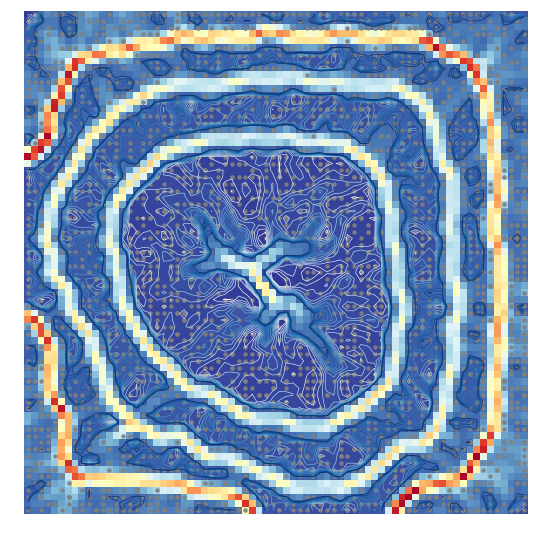
\includegraphics[scale=0.3]{SOM}
\caption{Non-globular dataset}\label{Ex-Fig1}

\end{figure}

In our initial experimental results in Figure~\ref{Ex-Fig2} conducted on topically labelled Airline tweets ($\approx$ 14,000 tweets) suggests SOM improves LDA significantly.

\begin{figure}[h]
	
	\centering 
	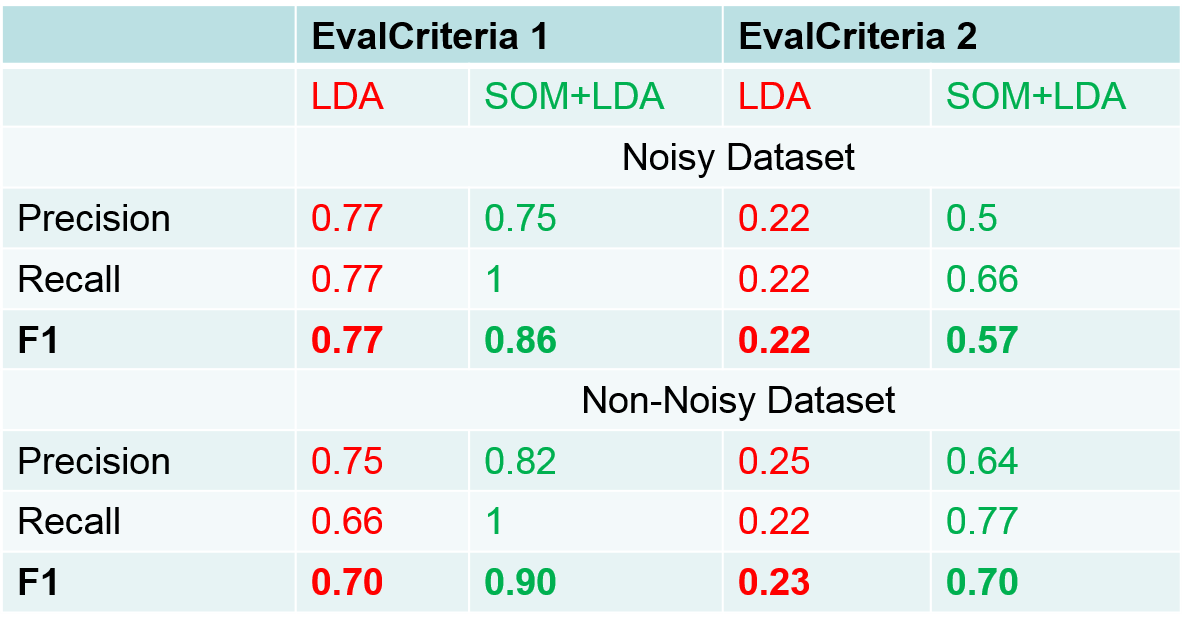
\includegraphics[scale=0.5]{PrelimExp1}
	\caption{Labelled Airline Tweets Topic Modelling}\label{Ex-Fig2}
	
\end{figure}

\subsection{Parameter Estimation}
The two most important parameters that need specifying are the map size for the SOM and the number of topics for LDA. We adopt the following strategies for specifying these parameters.

\subsubsection{Map Size}
With regards to the map size, we have established that the map size relates to the number of documents as well as the vocabulary size. In this preliminary report we assume the vocabulary remains constant and only discuss the observatory relationship between the number of documents and the map size. 

We begin by discussing the popularly known formula for determining a map size given by Vesanto~\cite{Vesanto00} as $NC=5\sqrt{n}$, where NC is the number of cells in the map and $n$ is the number of documents. The aim of this formula is to reduce the amount of empty cells. An empty cell means that when the dataset is projected unto the matrix, no data point is assigned to that cell. It is generally accepted that maps with fewer empty cells tend to be better. This may be true if the goal is to make inferences from the map visualisation. 

From our experiments, we observe that while smaller maps (maps with fewer empty cells) tend to give reasonable topics, the topics are often broad and its interpretations can be challenging. On the other hand, when the maps are bigger, we tend to have topics that are more specific. We can attribute this observation to the fact that, the clusters of the cells become more well defined. In each iteration of the training process, the BMU for each input document tends to be the same and far apart from another document's  BMU. In this way, each iteration enhances the closely co-occurring words in that BMU and diminishes the rarer co-occuring words. When the map is smaller, the BMU of each document are relatively closer, this means that the adjustments of one BMU are likely to influence the other BMU. From this we propose a somewhat heuristic solution to determining the best map size, following the same formula above but with a different interpretation. 

In place of the formula $5\sqrt{n}$, we propose $k\sqrt{n}$ where $k\in[5,{n}]$ and call $k$  a tuning parameter. This tuning parameter determines the specificity of topics \emph{i.e.} when  $k = {n}$, then the topics  become more specific and less specific when $k = 5$.  
Generally we notice that when $k=\frac{1}{10} \times n$ the results are very interpretable.

Figure \ref{Fig-SOM} shows how the maps change for different mapsizes with the same input data. In this experiment we used 670 tweets of the labelled airline dataset for a single day (24/02/2015). From the results we observe that as the map sizes increases the clusters of the cells in the map become more well defined. Table \ref{Tab-SOMSizes} shows the accompanying topics discovered. In the table we see that as the map sizes increases the topics become more specific. 

While the results here are inconclusive, it gives us an indication of the relationship between the map sizes, the dataset size and the topics discovered. This relationship will be explored further towards the writing of a scientific paper.

\begin{figure*}[htbp]
	\begin{minipage}[t]{0.47\linewidth}
		\begin{subfigure}{1\linewidth}
			\centering 
			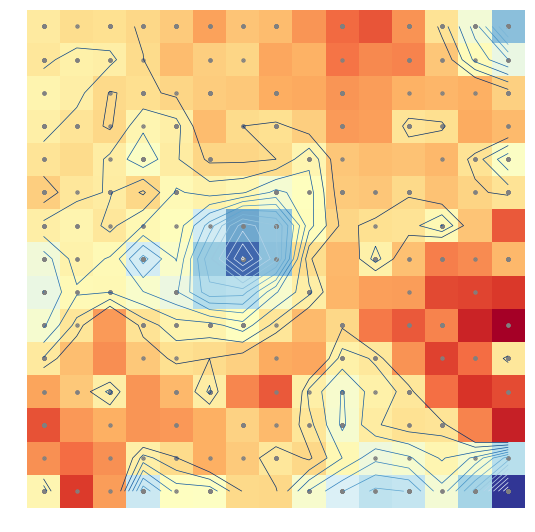
\includegraphics[scale=0.3]{SOM15x15}
			\caption{\centering 15 x 15 SOM }
			\label{Fig-SOM15}
		\end{subfigure}
	\end{minipage}
	\begin{minipage}[t]{0.47\linewidth}
	\begin{subfigure}{1\linewidth}
		\centering 
		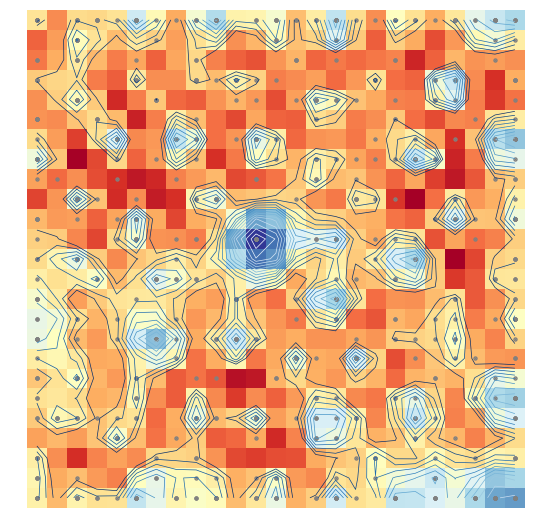
\includegraphics[scale=0.3]{SOM25x25}
		\caption{\centering 25 x 25 SOM}
		\label{Fig-SOM25}
	\end{subfigure}
	\end{minipage}

	\begin{minipage}[t]{0.47\linewidth}
	\begin{subfigure}{1\linewidth}
		%%%\vspace*{-2ex}
		\centering 
		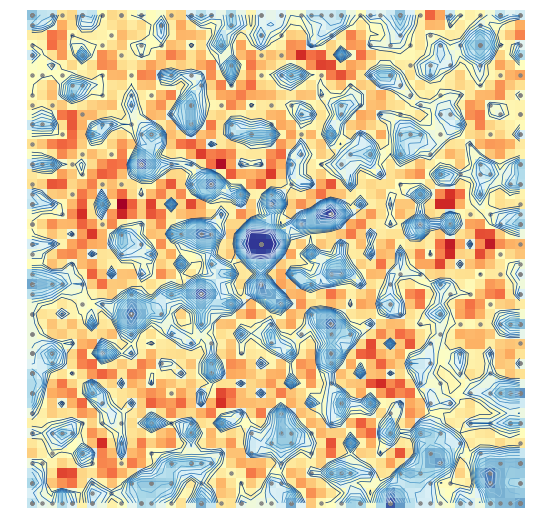
\includegraphics[scale=0.3]{SOM50x50}
		%\vspace*{-5ex}
		\caption{\centering 50 x 50 SOM}
		\label{Fig-SOM50}
	\end{subfigure}
	\end{minipage}
	\begin{minipage}[t]{0.47\linewidth}
	\begin{subfigure}{1\linewidth}
		\centering 
		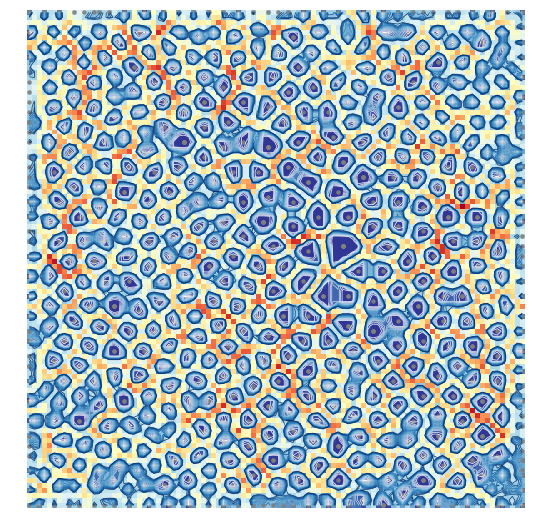
\includegraphics[scale=0.3]{SOM100x100}
		\caption{\centering 100 x 100 SOM}
		\label{Fig-SOM100}
	\end{subfigure}
\end{minipage}

\caption{Different SOM map sizes for the same input dataset}
\label{Fig-SOM}
\end{figure*}


\begin{table}[htbp]
\caption[title of table]{Topics Discovered for different Map sizes} \label{Tab-SOMSizes}
\centering

\begin{tabular}{|p{1.5cm}|p{10cm}| } % ccc means 3 columns, all centered; alternatives are l, r
	\hline
	&   \bf Topic Discovered and Keywords  \\ 
	\hline % draws a line under the column headers
	
	$15 \times 15 $ & ['wait', 'line', 'care', 'miss', 'need', 'travel', 'way'],
	
	['time', 'need', 'wait', 'travel', 'like', 'days', 'ive', 'tell', 'know', 'hold', 'phone', 'book', 'number', 'say', 'use', 'ask', 'try', 'agent', 'hours', 'dm', 'really', 'upgrade', 'flight', 'today', 'person', 'change', 'line', 'airport', 'make', 'help', 'people', 'luggage', 'online'],
	
	['flight', 'need', 'airport', 'wait', 'today', 'say', 'ive', 'make', 'agent'], 
	['problems', 'travel'], 
	
	['days', 'thank', 'say', 'cancel', 'seat', 'time', 'miss', 'need', 'dm', 'flightled', 'rude', 'want', 'work', 'wait', 'come', 'fly', 'tell', 'like', 'today', 'flight', 'response', 'luggage', 'book', 'make'], 
	
	['luggage', 'rude', 'lose', 'say', 'days', 'time']  \\
	\hline
	$25 \times 25 $&  ['aa', 'seat', 'book', 'like', 'work', 'upgrade', 'check'],
	
	['cancel', 'flight', 'fly', 'make'],
	
	['really', 'know', 'ask', 'like', 'tell'],
	
	['usairways', 'good', 'service'], 
	
	['delay', 'flight'], 
	
	['service', 'point', 'customer', 'ago'],
	
	['hold', 'try']   \\
	\hline
	$50 \times 50 $& ['seat'],
	 
	['bag', 'say'], 
	
	['ive', 'hold', 'min'], 
	
	['delay'], 
	
	['book'], 
	
	['miss', 'make', 'dont'], 
	
	['board', 'plane', 'sit', 'plan', 'late'], 
	
	['service', 'change', 'minutes'], 
	
	['flight', 'cancel']\\
	\hline
	$100 \times 100 $& ['hold'],
	 
	['tell', 'leave', 'hrs', 'phone'],
	 
	['cancel', 'flight'], 
	
	['aa', 'really'], 
	
	['board', 'dont', 'late', 'sit', 'lose', 'plan', 'miss'],
	
	['today', 'agent'], 
	
	['service'], 
	
	['book', 'flight', 'change', 'hour'], 
	
	['say', 'like', 'airport']\\
	\hline

	
\end{tabular}
\end{table}

\subsubsection{Number of Topics }

In all our experiments so far we use the known true number of topics in the dataset. However we strongly believe there is a relationship between the dense clusters (represented in blue) in the map and the actual number of topics.

From the literature we know that specifying a larger number of topics than the true number of topics has less detrimental results than specifying a smaller number of topics~\cite{Griffiths04}. The reason is that for a larger number of topics specified, the iterative process in LDA eventually obtains the dominant topics \emph{i.e.} the topic-word distribution of the extraneous topics is not supported by any document. Our aim here is to determine some lower bound on the number of topics required by LDA such that any number of topics specified greater than the lower bound yields reasonable results. 

So far, it seems that for the airline dataset, the best map size is anywhere between 25x25 to 50x50. For this range the best number of topics is 10. This means that if we can determine the map size ( either through the required specificity) then we can work out a good number (or range for the number of topics). However this needs to be further studied.

My aim is to use an approach similar to the elbow method used to determine the number of clusters of the k-means clustering method.

\subsubsection{Updating for Topic Evolution}
Our use of SOM makes updates relatively easier. In this sense, we train an initial SOM with training data. This map is then used to discover topics within the training dataset. The SOM is stored and when new tweets become available, the map is updated with the new tweets and then  topics rediscovered from the updated maps. Here, this has a few benefits but first I will clarify a few points. When we discover the topics from the updated SOM we will also discover some of the older topics, however this does not affect the goodness of our results because we only consider topics that are supported by the newly added documents \emph{i.e.} even though we still find some of the older topics if no documents support (are closely related to) those topics, they are discarded. This is as a direct result of the fact that only cells in the map that are closely related to the new set of documents will be activated, the remaining cells remain the same. 

A few advantages (but not all) of this approach is that we will always have a constant time operation w.r.t. the input dataset size since the map size remains constant (albeit the vocabulary may change). Also we do not need to re-cluster the whole dataset nor specify a different number of topics parameter for the new documents.


\section{Risk Analysis}
In this section we describe how we calculate the risk for each topic discovered by  our topic modelling approach. The overall idea here is that for each day, we discover the topics for the day and for each topic we identify the documents that relate to that topic and then calculate four factors from those documents. These factors are the aggregated sentiment score, polarity ratio, the gradient and the tweetrate. 

First, we find the harmonic mean between the polarity ratio and the aggregated sentiment score. This gives us an intermediary score. Let's call this score riskscore 1. We use the harmonic mean because the two values that we compare have different interpretations. The sentiment score reflects the feeling of people towards that topic. Since our goal here is to model the risk w.r.t the occurrence of a civil unrest, we only consider topics with an negative (bad) sentiment. The polarity ratio is the ratio of negative documents to the total count. This reflects whether a significant portion of the documents (people) are negative towards the topic or not. Using this intermediary riskscore 1, we can calculate the gradient between any two time intervals for that same topic. The gradient reflects how the riskscore 1 is growing. A high growth rate indicates that there is a surge in a negative interest in that topic and vice versa. This gradient is then combined with the intermediary riskscore 1 by harmonic mean to get the intermediary riskscore 2.  Finally we combine the riskscore 2 with the tweetrate by geometric mean to give a final riskscore value. Here the tweetrate gives an indication of the shear population size that are interested in this topic. We use a geometric mean because the two values have different interpretations and the ranges of the values can be significantly different.

For each day, we sum up the scores for all topics and compare daily score to gsr events. In this way we have a dataset with two columns. The first column is the riskscore column (predictor) and the second is the gsr event column (binary target). We train a logistic model with this data and then use it to determine the probability of an event occurring. In training the model we map the predictor values to the target values  by considering a lead time window. For example if we use a lead time window of 0 then it means we map the predictor value for each day to the target value of that same day. If the window is 2, then we map the predictor value to that day plus the target values for the following 2 days and  so on.

Our initial experiments on the freeport dataset shows that the results are quite reasonable. In this experiment we used 8 weeks of data. We trained the logistic model on the first 4 weeks and then used it to issue predictions for each day in the following 4 weeks. The predictions reflect the probability of an event occurring in a 2 day window from the day under consideration.  Figure \ref{Ex-Fig3} gives the results. Since the logistic regression gives a probability of an event, we need to specify thresholds beyond which we consider an event will happen. In this experiment, we consider 3 thresholds, $51\%$, $60\%$ and $70\%$ above which we consider a probability to mean an event will occur within the next 2 days. In the table we see that the precision is always perfect, this means each predicted event is correct. The recall seems reasonable but we believe this can even be improved if we train the logistic model on the scale of the events rather than the mere binary occurrence. This is because the predictor score that we calculate really reflects a scale rather than a binary value.

\begin{figure}[h]
	
	\centering 
	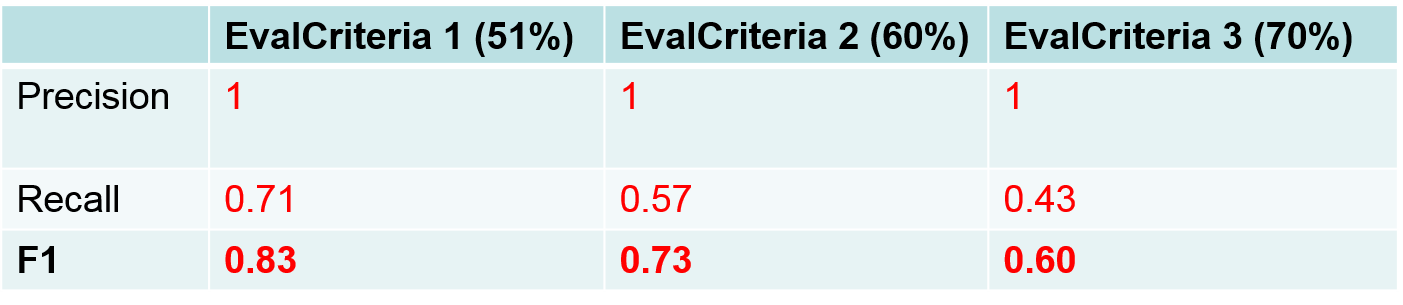
\includegraphics[scale=0.5]{PrelimExp2}
	\caption{Event Prediction from Freeport Dataset}\label{Ex-Fig3}
	
\end{figure}

Finally I would like to mention that we know that using the combined risk score value from the independent features gives better results than merely using the features independently as predictors. In current work, we are testing this to see the extent of improvement so that this can be recorded for the research paper.

   
\begin{thebibliography}{1}
 \bibitem{Blei03} David M. Blei, Andrew Y. Ng, Michael I. Jordan {\em Latent Dirichlet Allocation} Journal of Machine Learning Research, 2003.
 
 \bibitem{Kohonen82} Teuvo Kohonen {\em Self-Organized Formation of Topologically Correct Feature Maps} Biological Cybernetics, 1982.
 
 \bibitem{Griffiths04} Griffiths, T. L. Steyvers, M. {\em Finding Scientific Topics} Proceedings of the National Academy of Sciences, 2004.
 
 \bibitem{Vesanto00} Vesanto, J., Alhoniemi E. {\em Clustering of the Self-Organizing Map} IEEE Transactions on Neural Networks, Vol 11, N0.3, 2000.
\end{thebibliography}
\end{document}